
\documentclass[11pt,a4paper,openany]{report}
\usepackage[T1]{fontenc}
\usepackage[utf8]{inputenc}
\usepackage{lmodern}
\usepackage{microtype}
\usepackage{amsmath,amssymb,amsthm,mathtools,bm}
\usepackage{booktabs,array,longtable,tabularx}
\usepackage{xcolor}
\usepackage[margin=22mm,headheight=23pt]{geometry}
\usepackage{enumitem}
\usepackage{fancyhdr}
\usepackage{fancyvrb}
\usepackage{graphicx}
\usepackage{url}
\usepackage{xurl}
\usepackage{hyperref}
\definecolor{finblue}{HTML}{1F5A99}
\definecolor{fingreen}{HTML}{19733A}
\definecolor{finorange}{HTML}{D55E00}
\definecolor{finred}{HTML}{A61B1B}
\definecolor{finviolet}{HTML}{6A3D9A}
\definecolor{fingray}{HTML}{4D4D4D}

\hypersetup{
  unicode=true,colorlinks=true,linkcolor=finblue,citecolor=fingreen,
  urlcolor=finblue,
  pdftitle={FIN Local Research Checkpoint P454--P457},
  pdfauthor={Krzysztof Żuchowski},
  pdfsubject={Certified nested comb dual, ordered-symmetry obstruction, and six-decimal global cover},
  pdfkeywords={FIN, quantum comb, semidefinite duality, rational certificate, causal tester, symmetry obstruction, heralded erasure, interval cover}
}
\pagestyle{fancy}
\fancyhf{}
\fancyhead[L]{\small FIN Checkpoint P454--P457}
\fancyhead[R]{\small Release 10.41}
\fancyfoot[C]{\thepage}

\setlength{\parindent}{0pt}
\setlength{\parskip}{0.55em}
\setlist{nosep,leftmargin=2em}
\setcounter{tocdepth}{2}
\setcounter{secnumdepth}{3}
\emergencystretch=3em
\newcommand{\one}{\bm 1}
\newcommand{\C}{\mathbb C}
\newcommand{\R}{\mathbb R}
\newcommand{\Z}{\mathbb Z}
\newcommand{\statusProven}{\textcolor{fingreen}{[Proven]}}
\newcommand{\statusStrong}{\textcolor{finblue}{[Strong evidence]}}
\newcommand{\statusModerate}{\textcolor{finviolet}{[Moderate evidence]}}
\newcommand{\statusWeak}{\textcolor{fingray}{[Weak evidence]}}
\newcommand{\statusSpeculative}{\textcolor{finorange}{[Speculative]}}
\newcommand{\statusRefuted}{\textcolor{finred}{[Refuted]}}

\begin{document}
\hypersetup{pageanchor=false}
\begin{titlepage}
\centering
\vspace*{8mm}
{\Large\bfseries FIN Local Research --- Release 10.41\par}
\vspace{10mm}
{\Huge\bfseries Checkpoint P454--P457\par}
\vspace{6mm}
{\Large A Certified Nested Comb Dual, an Ordered-Symmetry Obstruction,\
and a Six-Decimal Global Cover\par}
\vspace{14mm}
{\Large Krzysztof \.Zuchowski\par}
\vspace{2mm}
{\normalsize Independent Researcher --- Fractal Information Theory Project\par}
\vspace{2mm}
{\normalsize ORCID: 0009-0002-0909-3613\par}
\vspace{8mm}
{\large 1 August 2026\par}
{\normalsize Publication --- Preprint; Version 1.0.0\par}
\vfill
\begin{minipage}{0.92\textwidth}
\small
\textbf{Central result.}
An explicit rational nested-dual certificate and the inherited coherent
primal witness confine the global three-slot causal half-distance to
\[
0.52332810026048937\le D_3^{\rm global}\le0.523334700252,
\]
a rigorous gap below $6.6\times10^{-6}$.

\medskip
\textbf{Additional results.}
Known ordered-comb symmetries leave a five-dimensional fixed space and cannot
force the three-dimensional coherent ansatz. A new globally licensed interval
cover confines the coarse erasure optimum to a gap below $10^{-6}$.

\medskip
\textbf{Boundary.}
No exact optimizer, optimizer uniqueness, selector, dimensional source,
laboratory record, complete legacy--strict bridge, role transfer, or physical
closure is claimed.

\medskip
\textbf{License.} CC BY 4.0.
\end{minipage}
\vfill
\end{titlepage}
\hypersetup{pageanchor=true}
\pagenumbering{roman}
\chapter*{Publication statement}
\addcontentsline{toc}{chapter}{Publication statement}
This monograph reports local analytical and computer-assisted Programs P454,
P455, and P457. It uses no laboratory record, external audit, internet result,
remote computation, or physical validation.
\tableofcontents
\clearpage
\pagenumbering{arabic}

\chapter{Executive summary}

This checkpoint completes local Programs P454, P455, and P457. It uses only analytical derivation, finite-dimensional linear algebra, rational arithmetic, directed intervals, and deterministic local optimization. It contains no laboratory data, external audit, internet result, remote computation, or physical evidence.

The three programs produce the following results.

\begin{enumerate}
\item 
\textbf{P454 --- [Proven /\allowbreak{} Computer-assisted proof].} The complete three-slot causal discrimination problem from P451 is written as a primal semidefinite program and a nested dual with matrix sizes

\[
   8\longrightarrow4\longrightarrow2\longrightarrow1.
   \]

A dependency-free log-determinant central-path scout locates a dual near the primal value. All entries are then rounded to explicit rationals. Six matrix slacks and two scalar slacks are certified strictly positive using exact Sylvester criteria. The two trigonometric slacks retain a margin greater than \(4.9999999969\times10^{-7}\) after paying the full operator perturbation. Together with the inherited P451 coherent primal witness, this proves the global full-cone bracket

\[
   0.52332810026048937
   \le D_3^{\rm global}
   \le0.523334700252.
   \]

Its exact width is

\[
   0.00000659999151063.
   \]

The corresponding success probability is confined to

\[
   0.761664050130244685
   \le p_{\rm succ}^{\rm global}
   \le0.761667350126.
   \]

\item 
\textbf{P455 --- [Proven /\allowbreak{} Strong evidence].} The complex three-slot causal cone has 21 affine dimensions. Complex conjugation and global bit complement can be averaged because the objective is concave and invariant, so an optimizer has a real, complement-fixed representative. The real cone has 14 affine dimensions. Exact finite rank gives nine independent complement constraints and a five-dimensional fixed space. The O167 coherent ansatz has only three dimensions. Therefore two symmetry-allowed directions remain, and known symmetries alone cannot prove reduction to O167. This is a rigorous obstruction to the proposed symmetry shortcut. Eight deterministic searches over all five fixed dimensions return to the O167 value within \(6.7\times10^{-16}\), with a negative sampled Hessian, but this non-improvement remains strong evidence rather than a theorem.

\item 
\textbf{P457 --- \textcolor{fingreen}{[Computer-assisted proof]}.} P452 already licensed reversal reduction of the exact coarse erasure objective to the palindromic line. P457 performs a new outward-rounded cover at tolerance \(10^{-6}\). The cover evaluates 5,008 boxes and terminates with

\[
   0.463278283192093
   \le D_{\rm coarse}^{\rm global}
   \le0.46327928294340853,
   \]

whose width is

\[
   9.997513155113325\times10^{-7}.
   \]

This is a factor of approximately 992.7 narrower than the Release-10.40 bound.

\end{enumerate}

The checkpoint constructs three typed objects:

\begin{itemize}
\item 
\textbf{O170 --- Nested Comb Dual Ladder;}

\item 
\textbf{O171 --- Ordered-Comb Symmetry Residual Space;}

\item 
\textbf{O172 --- Six-Decimal Coarse-Erasure Cover.}

\end{itemize}

No exact P454 optimizer, optimizer uniqueness, selector, canonical physical orientation, dimensional unit, apparatus, laboratory record, complete legacy-to-strict bridge, role-transfer theorem, Standard Model, gravity theory, \(L_{\rm total}\), or Theory of Everything is claimed.

\par\medskip\hrule\medskip

\chapter{Confidence convention}

\begin{center}
\begingroup\small
\setlength{\tabcolsep}{2.5pt}
\renewcommand{\arraystretch}{1.16}
\begin{longtable}{@{}p{0.420\textwidth}p{0.420\textwidth}@{}}
\toprule
\textbf{Label} & \textbf{Meaning} \\
\midrule
\endhead
\statusProven{} & Exact analytic or finite algebraic result under declared premises \\
\textcolor{fingreen}{[Computer-assisted proof]} & Finite rational/\allowbreak{}interval certificate with auditable code and artifacts \\
\statusStrong{} & Deterministic numerical agreement and falsification tests without a complete certificate \\
\textcolor{finviolet}{[Conditional]} & Result depends on an explicitly supplied interface or variational rule \\
\textcolor{finorange}{[Open]} & Current artifacts do not decide the proposition \\
\textcolor{finred}{[Blocked by external evidence]} & A laboratory, calibration, custody, or external record is indispensable \\
\bottomrule
\end{longtable}
\endgroup
\end{center}

\par\medskip\hrule\medskip

\chapter{Inherited assumptions and state map}

\section{Inputs retained from Release 10.40}

\begin{itemize}
\item 
P449 gives the exact compressed causal recursion

\[
  \mathcal C_n=
  \{B_0\oplus B_1:\ B_0,B_1\succeq0,
  \ B_0+B_1\in\mathcal C_{n-1}\}.
  \]

\item 
P451 gives the certified rational coherent primal witness with

\[
  D_{\rm primal}\ge0.52332810026048937.
  \]

\item 
P452 proves reversal symmetrization of the declared actual coarse erasure objective, not merely its fine-label majorant.

\item 
P446 provides the outward one-dimensional branch procedure reused in P457.

\item 
P453 proves uniqueness of the minimum-negative-mass signed representation, conditional on its inherited certified inputs.

\end{itemize}

\section{State map}

\begin{center}
\begingroup\small
\setlength{\tabcolsep}{2.5pt}
\renewcommand{\arraystretch}{1.16}
\begin{longtable}{@{}p{0.218\textwidth}p{0.348\textwidth}p{0.293\textwidth}@{}}
\toprule
\textbf{Lane} & \textbf{State before this checkpoint} & \textbf{New state} \\
\midrule
\endhead
Three-slot causal optimum & Primal lower \(0.52332810026048937\); full optimum open & Rigorous global upper \(0.523334700252\); gap \(<6.7\times10^{-6}\) \\
Coherent symmetry face & Three-parameter O167 candidate & Five-dimensional exact fixed space; two residual directions proved \\
Coarse erasure code & Full-simplex gap \(<10^{-3}\) & Full-simplex gap \(<10^{-6}\) \\
P453 canonical gauge & Unique only inside minimum-TV rule & Unchanged \\
Selector/\allowbreak{}QW-2191 & Open & Unchanged \\
Dimensional source & Missing & Unchanged \\
Laboratory evidence & None & None \\
Legacy-to-strict bridge & Incomplete & Unchanged \\
\bottomrule
\end{longtable}
\endgroup
\end{center}

\section{Kernel and ontology guardrails}

The intermediate and strict kernels remain distinct:

\[
K_{\rm legacy,ont}(d)=
\frac{\alpha_{\rm geo}\cos(\omega d+\phi)}{1+\beta_{\rm tors}d},
\]

\[
K_{\rm strict,gate}(d)=
\frac{\cos(\omega d+\phi)}{1+\beta d^\eta}.
\]

Kernel new Legacy /\allowbreak{} Legacy* remains a researched historical/\allowbreak{}intermediate bridge subclass and is not silently substituted for the strict kernel. The present programs are downstream reduced-channel calculations. They derive neither kernel and transfer no legacy physical role.

The internal ontology remains

\[
\text{nadsoliton}\to\text{light}\to\text{matter}
\to\text{emergent observer},
\]

with no lower informational layer beneath the nadsoliton.

\par\medskip\hrule\medskip

\chapter{Program P454 --- exact nested comb dual and global bracket}

\section{Exact question}

Can the full 21-dimensional three-slot causal optimization left open by P451 receive a matching rigorous upper bound without installing an external SDP package or treating a floating optimizer as a theorem?

\section{Primal SDP}

Let \(\Delta=\Delta_3\) be the supplied eight-dimensional compressed process difference. Introduce positive measurement testers \(T_+,T_-\succeq0\) and positive causal-normalization layers

\[
B_0,B_1\in\mathbb H_+^4,
\qquad
C_0,C_1\in\mathbb H_+^2,
\qquad
d_0,d_1\ge0.
\]

The primal is

\[
\begin{aligned}
\text{maximize}\quad &
\frac12\operatorname{Tr}\!\left[\Delta(T_+-T_-)\right]\\
\text{subject to}\quad &
T_++T_-=B_0\oplus B_1,\\
&B_0+B_1=C_0\oplus C_1,\\
&C_0+C_1=\operatorname{diag}(d_0,d_1),\\
&d_0+d_1=1.
\end{aligned}
\]

For fixed normalization \(N=T_++T_-\), binary Helstrom optimization gives

\[
\max_{T_\pm}\frac12\operatorname{Tr}[\Delta(T_+-T_-)]
=\frac12\lVert N^{1/2}\Delta N^{1/2}\rVert_1.
\]

Thus the SDP is exactly the P451 full-cone objective, not a relaxation.

\section{Dual derivation}

Introduce Hermitian multipliers

\[
X_3\in\mathbb H^8,
\quad X_2\in\mathbb H^4,
\quad X_1\in\mathbb H^2,
\]

and scalar \(\lambda\). Taking the supremum over every positive primal variable is finite precisely when

\[
X_3\succeq\frac{\Delta}{2},
\qquad
X_3\succeq-\frac{\Delta}{2},
\]

\[
X_2\succeq (X_3)_{00},
\qquad
X_2\succeq (X_3)_{11},
\]

\[
X_1\succeq (X_2)_{00},
\qquad
X_1\succeq (X_2)_{11},
\]

\[
\lambda\ge(X_1)_{00},
\qquad
\lambda\ge(X_1)_{11}.
\]

Here the subscripts denote the two equal-size principal blocks at the next causal level. The dual is

\[
\text{minimize}\quad\lambda.
\]

This produces the new hierarchy

\[
\boxed{X_3\to X_2\to X_1\to\lambda},
\]

which is O170.

Both sides possess strict feasible points: the central normalized tester is strictly primal feasible after a strictly positive outcome split, and large scalar identities are strictly dual feasible. Finite-dimensional Slater duality therefore applies. Weak duality alone already suffices for the certified upper bound.

\section{Dependency-free locator}

No local cvxpy, cvxopt, SCS, Clarabel, or commercial SDP solver is available. P454 therefore uses the local barrier

\[
\Phi_\mu=
\lambda-\mu\sum_{j=1}^{8}\log\det S_j,
\]

where \(S_j\) are the six matrix and two scalar dual slacks. Complex conjugation swaps the first two constraints, so the dual variables can be chosen real symmetric while \(\Delta\) remains imaginary Hermitian.

A deterministic feasible BFGS method with explicit Armijo backtracking follows twelve barrier values from \(10^{-1}\) to \(3\times10^{-7}\). The last point has

\[
\lambda_{\rm scout}=0.5233347002511172.
\]

The last barrier iteration does not meet the chosen gradient tolerance. It is used only to locate rational matrices and is never itself the certificate.

\section{Rationalization and exact positivity}

Every entry of \(X_3,X_2,X_1\) is rounded to denominator \(10^{12}\), and \(\lambda\) is rounded upward:

\[
\lambda_{\mathbb Q}
=\frac{130833675063}{250000000000}
=0.523334700252.
\]

The entries of \(\Delta/2\) are enclosed by the inherited rational Machin/\allowbreak{}Taylor provider and rounded to denominator \(10^{20}\). The maximum entry radius is paid using

\[
\lVert E\rVert_2\le8\max_{ij}|E_{ij}|.
\]

For each rational midpoint matrix slack \(S\), exact Sylvester tests are applied to

\[
S-\frac{1}{2\,000\,000}I.
\]

All leading principal minors are strictly positive:

\begin{itemize}
\item 
eight for each \(8\times8\) trigonometric slack;

\item 
four for each \(4\times4\) inherited slack;

\item 
two for each \(2\times2\) inherited slack;

\item 
one for each scalar slack.

\end{itemize}

The trigonometric operator perturbation is only

\[
3.0514767686602317\times10^{-16},
\]

so the certified exact minimum-eigenvalue lower bound for each top slack is

\[
4.9999999969485233\times10^{-7}>0.
\]

The other matrix slacks retain the exact margin \(1/2{,}000{,}000\), and the two scalar slacks are approximately \(5.99997\times10^{-7}\) and \(5.99995\times10^{-7}\). Thus the rational dual is strictly feasible.

\section{Global theorem and limitation}

Combining the P451 primal lower bound and P454 dual upper bound gives

\[
0.52332810026048937
\le D_3^{\rm global}
\le0.523334700252.
\]

The exact gap is

\[
\frac{659999151063}{10^{17}}
=6.59999151063\times10^{-6}.
\]

\textbf{P454 verdict:} the nested dual derivation is \textbf{\statusProven{}}, and the rational upper bound plus global bracket are \textbf{\textcolor{fingreen}{[Computer-assisted proof]}}. Exact attainment by O167 and optimizer uniqueness remain \textbf{\textcolor{finorange}{[Open]}}.

\par\medskip\hrule\medskip

\chapter{Program P455 --- ordered-comb symmetry residual space}

\section{Exact question}

Can the three-parameter O167 face be derived from the symmetries already present in the ordered three-slot cone, thereby converting its numerical optimum into the full optimum?

\section{Real causal tangent space}

The P449 complex Hermitian affine dimension is 21. Because

\[
D(N)=D(\overline N)
\]

and \(D\) is concave, averaging \(N\) with \(\overline N\) cannot lower the objective. Hence a real-symmetric optimizer exists.

The exact real affine recursion has dimension

\[
e_1=1,
\qquad e_n=e_{n-1}+\frac{2^{n-1}(2^{n-1}+1)}{2}.
\]

For three slots,

\[
e_3=1+3+10=14.
\]

An explicit integer basis consists of one last-level diagonal direction, three real-symmetric \(C_0\) directions, and ten real-symmetric \(B_0\) directions.

\section{Global complement}

Let \(J_8\) reverse all three history bits. The objective is invariant under the induced global-complement action. Averaging with

\[
N\mapsto J_8NJ_8
\]

again cannot lower a concave invariant objective.

On the exact fourteen-direction integer basis, the linear constraints

\[
J_8NJ_8=N
\]

have rank nine. Therefore the real, complement-fixed affine space has

\[
14-9=5
\]

dimensions. The computation exports five exact nullspace vectors with entries in \(\{-1,0,1\}\).

\section{Why O167 is not symmetry-forced}

The O167 form

\[
N(A,B,u)=B_0(A,B,u)\oplus B_1(A,B,u),
\]

with

\[
C=\frac12-A-2B
\]

has only three independent affine directions. Direct rank computation proves that this face is contained in the five-dimensional fixed space but does not fill it. The residual dimension is

\[
5-3=2.
\]

Thus complex conjugation plus global complement do not imply the O167 ansatz. Any proof of that reduction needs one additional invariant, a KKT theorem, a dual complementary-slackness argument, or an independent source law.

This is a rigorous obstruction, not a failed numerical search.

\section{Falsification in all five dimensions}

The O167 face optimization gives

\[
(A,B,u)=
(0.28716641518022373,
0.068777213178814,
0.009493712418100549)
\]

and

\[
D_{\rm face}=0.5233281002710417.
\]

The minimum normalizer eigenvalue is \(0.0577235542\), so the point is well inside the positive region. Eight deterministic Nelder--Mead starts over all five fixed coordinates give values between

\[
0.5233281002710413
\quad\text{and}\quad
0.5233281002710424.
\]

The maximum apparent gain over the face is

\[
6.661338147750939\times10^{-16}.
\]

A finite-difference Hessian in the five-dimensional fixed space has sampled eigenvalues

\[
(-2.4559,-1.4969,-1.0050,-0.6617,-0.3045),
\]

all negative. This is strong, robust local evidence that the two residual directions do not improve the candidate. It is not a proof of global five-dimensional optimality.

\textbf{P455 verdict:} the five-dimensional fixed space and two-dimensional residual are \textbf{\statusProven{}}. Return to the O167 value is \textbf{\statusStrong{}}. The hypothesis that known symmetries alone force O167 is \textbf{\statusRefuted{}}.

\par\medskip\hrule\medskip

\chapter{Program P457 --- six-decimal full-simplex erasure cover}

\section{Exact question}

After P452 converted the P446 palindromic line into a theorem for the complete declared simplex, how much can the value bracket be tightened using the same auditable outward arithmetic without a new conceptual assumption?

\section{Licensed one-dimensional reduction}

P452 proves

\[
D_{\rm coarse}(p)
\le D_{\rm coarse}\!\left(\frac{p+p^{\rm rev}}2\right)
\]

at \(q=4/5\), \(\theta=2\pi/15\). Every reversal average has the form

\[
p(a)=(a,1/2-a,1/2-a,a),
\qquad0\le a\le1/2.
\]

P457 changes only the interval tolerance, from \(10^{-3}\) to \(10^{-6}\). No full-simplex point is omitted because P452 supplies the exact reduction.

\section{Finite cover}

The directed binary64 implementation expands every arithmetic primitive by one representable number. Each branch cell receives an interval upper bound; midpoint evaluations update a certified feasible lower bound. The run uses

\begin{itemize}
\item 
5,008 evaluated boxes;

\item 
5,009 terminal boxes;

\item 
deterministic initial interval \([0,1/2]\);

\item 
no stochastic pruning.

\end{itemize}

The final bracket is

\[
0.463278283192093
\le D_{\rm coarse}^{\rm global}
\le0.46327928294340853.
\]

The width is

\[
9.997513155113325\times10^{-7}<10^{-6}.
\]

The best certified point has

\[
a=0.2276921272277832,
\]

and the conservative live maximizer hull is

\[
[0.2178955078125,0.234619140625].
\]

The new gap is approximately 992.712 times smaller than the P452 gap.

\textbf{P457 verdict:} the full-simplex bracket is \textbf{\textcolor{fingreen}{[Computer-assisted proof]}}. A closed-form maximizer, uniqueness, unrestricted inputs, adaptivity, and laboratory performance remain \textbf{\textcolor{finorange}{[Open]}}.

\begin{figure}[htbp]
\centering
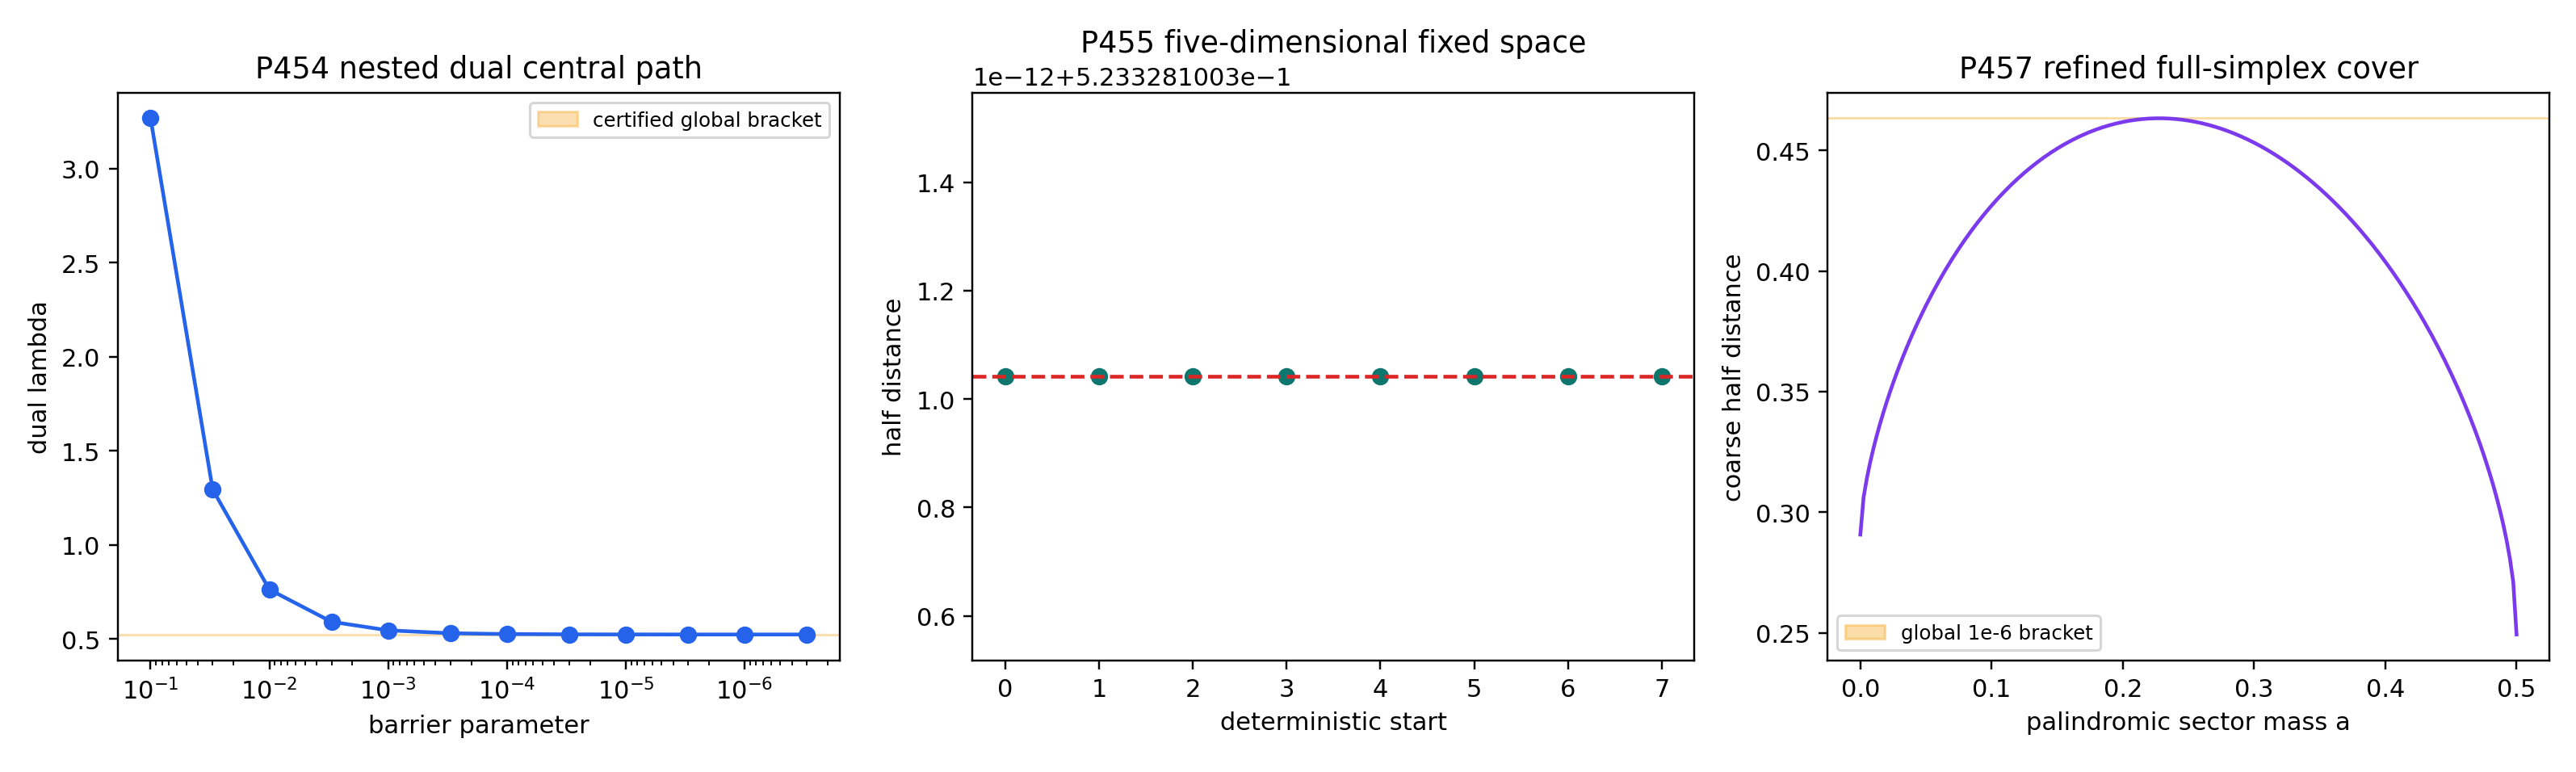
\includegraphics[width=0.97\textwidth]{FIN_Programs_454_455_457_Figures/p454_p457_dual_symmetry_and_refined_cover.png}
\caption{The nested-dual central path and certified global bracket, the five-dimensional ordered-symmetry audit, and the refined globally licensed coarse-erasure cover.}
\end{figure}

\par\medskip\hrule\medskip

\chapter{Newly constructed theoretical objects}

\section{O170 --- Nested Comb Dual Ladder}

\begin{center}
\begingroup\small
\setlength{\tabcolsep}{2.5pt}
\renewcommand{\arraystretch}{1.16}
\begin{longtable}{@{}p{0.420\textwidth}p{0.420\textwidth}@{}}
\toprule
\textbf{Required field} & \textbf{Definition and audit} \\
\midrule
\endhead
Name & Nested Comb Dual Ladder \\
Domain/\allowbreak{}codomain & Three-slot primal tester SDP \(\mapsto(X_3,X_2,X_1,\lambda)\) dual \\
Complete definition & The eight Loewner/\allowbreak{}scalar inequalities displayed in Section 4 \\
Premises & P449 causal recursion; declared reduced \(\Delta_3\) \\
Transformation law & Block levels follow the ordered causal trace hierarchy \\
Generated theorem & Global full-cone upper bound \(0.523334700252\) \\
Necessity test & A scalar norm bound cannot resolve the P451 coherence gap to \(10^{-5}\) scale \\
Removal attempt & Removing any level loses the corresponding causal normalization constraint \\
Strict/\allowbreak{}legacy relation & Downstream reduced channel; derives neither kernel and transfers no role \\
Selector dependence & Ordered slots are supplied; no QW-2191 discharge \\
Dimensional status & Dimensionless \\
Operational interpretation & Mathematical dual witness for binary causal discrimination \\
Failure mode & Does not prove exact optimizer or apparatus implementation \\
Confidence & \textbf{\statusProven{}} dual; \textbf{\textcolor{fingreen}{[Computer-assisted proof]}} rational certificate \\
\bottomrule
\end{longtable}
\endgroup
\end{center}

\section{O171 --- Ordered-Comb Symmetry Residual Space}

\begin{center}
\begingroup\small
\setlength{\tabcolsep}{2.5pt}
\renewcommand{\arraystretch}{1.16}
\begin{longtable}{@{}p{0.420\textwidth}p{0.420\textwidth}@{}}
\toprule
\textbf{Required field} & \textbf{Definition and audit} \\
\midrule
\endhead
Name & Ordered-Comb Symmetry Residual Space \\
Domain/\allowbreak{}codomain & Real \(\mathcal C_3\) tangent space \(\mapsto\ker(J_8(\cdot)J_8-I)\) \\
Complete definition & Exact rank-nine complement action on a fourteen-direction integer basis \\
Premises & Conjugation and global-complement invariance; causal order retained \\
Transformation law & Fixed under \(N\mapsto J_8NJ_8\) \\
Generated theorem & Fixed dimension five; O167 codimension two inside it \\
Necessity test & Explains why symmetry alone cannot close P451 exact globality \\
Removal attempt & Discarding the residual directions silently assumes two unproved constraints \\
Strict/\allowbreak{}legacy relation & Kernel-split robust downstream cone geometry \\
Selector dependence & Complement invariance distinguishes no orientation \\
Dimensional status & Dimensionless \\
Operational interpretation & Admissible ordered tester-normalization directions \\
Failure mode & Numerical non-improvement along residual directions is not a theorem \\
Confidence & \textbf{\statusProven{}} dimension; \textbf{\statusStrong{}} optimizer location \\
\bottomrule
\end{longtable}
\endgroup
\end{center}

\section{O172 --- Six-Decimal Coarse-Erasure Cover}

\begin{center}
\begingroup\small
\setlength{\tabcolsep}{2.5pt}
\renewcommand{\arraystretch}{1.16}
\begin{longtable}{@{}p{0.420\textwidth}p{0.420\textwidth}@{}}
\toprule
\textbf{Required field} & \textbf{Definition and audit} \\
\midrule
\endhead
Name & Six-Decimal Coarse-Erasure Cover \\
Domain/\allowbreak{}codomain & Palindromic \(a\in[0,1/2]\mapsto\) global objective bracket \\
Complete definition & Outward interval branch cover at tolerance \(10^{-6}\) \\
Premises & P452 full-simplex reversal theorem and declared P446 channel/\allowbreak{}code \\
Transformation law & Reversal invariant \\
Generated theorem & Global bracket width \(<10^{-6}\) \\
Necessity test & Reusing the old tolerance leaves a thousand-times wider uncertainty \\
Removal attempt & Floating maximization alone provides no global bound \\
Strict/\allowbreak{}legacy relation & Downstream, kernel-split robust after channel supply \\
Selector dependence & None; averaging does not select a direction \\
Dimensional status & Dimensionless; "six-decimal" is numerical, not a length scale \\
Operational interpretation & Mathematical code-performance certificate \\
Failure mode & Scope does not include arbitrary inputs, adaptive codes, or hardware \\
Confidence & \textbf{\textcolor{fingreen}{[Computer-assisted proof]}} \\
\bottomrule
\end{longtable}
\endgroup
\end{center}

\par\medskip\hrule\medskip

\chapter{Falsification and robustness audit}

\section{P454: no solver output was accepted as proof}

The last central-path point fails the selected gradient tolerance. The report does not hide this. Its only role is to locate rational matrices. The theorem uses exact rational entries, exact leading principal minors, an upward-rounded objective, and a separately paid transcendental perturbation.

\section{P454: global value is bounded, not identified exactly}

The primal and dual witnesses differ by \(6.6\times10^{-6}\). Nothing in duality says the O167 face attains the exact optimum until the gap is closed or complementary slackness is certified.

\section{P455: symmetry shortcut is rigorously insufficient}

The five-versus-three dimension count is exact. The two missing directions cannot be deleted because eight numerical starts did not exploit them. A new theorem must eliminate them or a future counterexample may use them.

\section{P455: local Hessian is not global concavity proof}

Although all five sampled Hessian eigenvalues are negative, the objective is concave in the normalizer but maximizing a concave function does not permit arbitrary conclusions from a sampled Hessian. A stationary supergradient or restricted dual is still required.

\section{P457: expensive cover is finite and scoped}

The 5,008-box run is deterministic and terminates. It does not justify repeating blind refinement indefinitely. The next conceptual move should isolate the derivative or prove uniqueness rather than merely add decimal places.

\par\medskip\hrule\medskip

\chapter{Reproducibility boundaries}

\begin{center}
\begingroup\small
\setlength{\tabcolsep}{2.5pt}
\renewcommand{\arraystretch}{1.16}
\begin{longtable}{@{}p{0.104\textwidth}p{0.253\textwidth}p{0.287\textwidth}p{0.215\textwidth}@{}}
\toprule
\textbf{Program} & \textbf{Proof-grade layer} & \textbf{Scout-only layer} & \textbf{Remaining boundary} \\
\midrule
\endhead
P454 & Exact dual derivation, rational matrices, Sylvester margins, interval perturbation & Barrier path & Exact optimizer and uniqueness \\
P455 & Exact dimension/\allowbreak{}rank/\allowbreak{}nullspace & Five-dimensional Nelder--Mead and Hessian & Eliminate or exploit two residual directions \\
P457 & Outward exhaustive 1D cover licensed by P452 & Plot sampling & Closed form and uniqueness \\
\bottomrule
\end{longtable}
\endgroup
\end{center}

The complete P457 batch takes approximately three minutes on the declared Intel i3-10110U system, dominated by interval evaluation. The P454 rational certificate is much cheaper than dense exact characteristic-polynomial isolation because Sylvester margins directly prove the required positivity.

\par\medskip\hrule\medskip

\chapter{Physical and epistemic boundary}

\begin{center}
\begingroup\small
\setlength{\tabcolsep}{2.5pt}
\renewcommand{\arraystretch}{1.16}
\begin{longtable}{@{}p{0.420\textwidth}p{0.420\textwidth}@{}}
\toprule
\textbf{Question} & \textbf{Status after P454--P457} \\
\midrule
\endhead
Mathematical three-slot tester value & Globally bracketed to \(<6.7\times10^{-6}\) \\
Physical preparation of that tester & Not established \\
Physical clock or dimensional time & Not generated \\
Vertex POVM /\allowbreak{} twelve-state apparatus & Not demonstrated \\
Laboratory event record & None \\
QW-2191 selector & Open \\
Canonical orientation or phase origin & Open \\
Information-to-thermodynamic entropy & Not established \\
Legacy-to-strict completion & Open \\
Legacy physical-role transfer & Not started \\
Standard Model, gravity, \(L_{\rm total}\), ToE & Not established \\
\bottomrule
\end{longtable}
\endgroup
\end{center}

The ordered causal hierarchy is a mathematical interface. It is not a physical arrow of time and does not source a Z12 orientation. The numerical parameter \(\mu\) in the barrier method is not a physical scale.

\par\medskip\hrule\medskip

\chapter{Ranked next research programs}

\begin{center}
\begingroup\fontsize{7}{8.4}\selectfont
\setlength{\tabcolsep}{2.5pt}
\renewcommand{\arraystretch}{1.16}
\begin{longtable}{@{}p{0.055\textwidth}p{0.086\textwidth}p{0.283\textwidth}p{0.261\textwidth}p{0.175\textwidth}@{}}
\toprule
\textbf{Rank} & \textbf{Program} & \textbf{Exact target} & \textbf{Cheapest decisive method} & \textbf{Probability of decisive local result} \\
\midrule
\endhead
1 & \textbf{P464} & Close or sharply reduce the P454 \(6.6\times10^{-6}\) primal--dual gap & Build a five-dimensional restricted dual/\allowbreak{}KKT inclusion using O171 &  \\
2 & \textbf{P458} & Prove or refute uniqueness of the P457 palindromic maximizer & Interval isolate the derivative and certify monotonicity cells &  \\
3 & \textbf{P459} & Propagate P453 global uniqueness through the full O163 detector box & Combine forced support with P447 interval allocation sensitivities &  \\
4 & \textbf{P460} & Construct a null-cycle-quotient estimator or prove a no-go & Linear invariant analysis on the degree-11 moment quotient &  \\
5 & \textbf{P461} & Formalize the P452 coefficient theorem & Lean proof with a typed cosine-positivity provider boundary &  \\
6 & \textbf{P462} & Formalize P453 support forcing and Vandermonde uniqueness & Lean finite-measure complementarity plus finite Vandermonde lemma &  \\
7 & \textbf{P463} & Freeze an executable preparation contract for O169 & Local schema, validator, synthetic integration test marked nonphysical &  \\
8 & \textbf{P465} & Produce a higher-precision rational O167 primal witness & Rationalize the face optimizer and repeat exact trace-distance certification &  \\
9 & \textbf{P466} & Test causal coherence at four slots & P449 recursion, global diagonal symmetry, one rational coherent witness &  \\
10 & \textbf{P467} & Generalize O170 to arbitrary slot number & Inductive primal/\allowbreak{}dual comb ladder theorem and dimension recurrence &  \\
\bottomrule
\end{longtable}
\endgroup
\end{center}

The selected next batch is

\[
\boxed{P464\longrightarrow P458\longrightarrow P459}.
\]

P464 attacks the most important remaining mathematical gap. P458 replaces further brute-force decimals with a uniqueness theorem or counterexample. P459 converts P453's canonical mathematical gauge into a fully propagated, still explicitly nonphysical operational design.

\par\medskip\hrule\medskip

\chapter{Exact artifact list}

\begin{itemize}
\item 
FIN\_Local\_Research\_Checkpoint\_P454\_P457\_EN.md

\item 
FIN\_Local\_Research\_Checkpoint\_P454\_P457\_EN.tex

\item 
FIN\_Local\_Research\_Checkpoint\_P454\_P457\_EN.pdf

\item 
FIN\_Current\_Local\_Research\_Report\_EN.pdf

\item 
FIN\_Local\_Research\_Checkpoint\_P454\_P457\_State.json

\item 
RELEASE\_10\_41\_PROGRAMS\_454\_455\_457.md

\item 
FIN\_Checkpoint\_P454\_P457\_AGENTS\_Guardrail.txt

\item 
FIN\_PROGRAMS\_454\_455\_457\_RELEASE\_MANIFEST.sha256

\item 
FIN\_Programs\_454\_455\_457\_Results.json

\item 
FIN\_Programs\_454\_455\_457\_Summary.csv

\item 
FIN\_Programs\_454\_455\_457\_P454\_Nested\_Dual.csv

\item 
FIN\_Programs\_454\_455\_457\_P454\_Rational\_Dual.npz

\item 
FIN\_Programs\_454\_455\_457\_P455\_Symmetry\_Residual.csv

\item 
FIN\_Programs\_454\_455\_457\_P457\_Refined\_Cover.csv

\item 
FIN\_Programs\_454\_455\_457\_Figures/\allowbreak{}p454\_p457\_dual\_symmetry\_and\_refined\_cover.png

\item 
fin\_programs\_454\_455\_457.py

\item 
fin\_programs\_454\_455\_457\_to\_latex.py

\item 
test\_fin\_programs\_454\_455\_457.py

\item 
test\_fin\_checkpoint\_p454\_p457.py

\end{itemize}

\par\medskip\hrule\medskip

\chapter{Restart instructions}

Run the bounded scientific batch:

\begin{Verbatim}[fontsize=\small]
MPLCONFIGDIR=/tmp/fin-mpl-1038 python3 fin_programs_454_455_457.py
\end{Verbatim}

Run current and inherited regression tests:

\begin{Verbatim}[fontsize=\small]
MPLCONFIGDIR=/tmp/fin-mpl-1038 python3 -m unittest -v \
  test_fin_programs_454_455_457.py \
  test_fin_checkpoint_p454_p457.py \
  test_fin_checkpoint_p451_p453.py
\end{Verbatim}

Regenerate and compile the monograph:

\begin{Verbatim}[fontsize=\small]
python3 fin_programs_454_455_457_to_latex.py
lualatex -interaction=nonstopmode -halt-on-error \
  FIN_Local_Research_Checkpoint_P454_P457_EN.tex
lualatex -interaction=nonstopmode -halt-on-error \
  FIN_Local_Research_Checkpoint_P454_P457_EN.tex
\end{Verbatim}

Verify the manifest:

\begin{Verbatim}[fontsize=\small]
sha256sum -c FIN_PROGRAMS_454_455_457_RELEASE_MANIFEST.sha256
\end{Verbatim}

Before P464, reread the latest AGENTS.md guardrail and do not promote the P455 numerical return to O167 into a symmetry theorem.

\par\medskip\hrule\medskip

\chapter{Final conclusion}

P454 changes the status of the three-slot causal problem from "one good coherent witness" to a globally bracketed finite SDP. P455 then explains why the remaining tiny gap cannot be erased by invoking the currently known symmetries: two exact ordered-comb directions survive outside O167. P457 shows that the separate coarse-erasure code problem is now controlled to six decimal places on its entire declared simplex.

The strongest interpretation surviving falsification is still purely mathematical: FIN supplies finite dimensionless operator, comb, and moment optimization problems that admit increasingly sharp primal, dual, symmetry, and variational certificates. None of these certificates supplies the missing bridge from mathematical information dynamics to experimentally testable dimensional physics.


\clearpage
\chapter*{Reproduction certificate}
\addcontentsline{toc}{chapter}{Reproduction certificate}
\begin{Verbatim}[fontsize=\small]
MPLCONFIGDIR=/tmp/fin-mpl-1038 \
python3 fin_programs_454_455_457.py

MPLCONFIGDIR=/tmp/fin-mpl-1038 \
python3 -m unittest -v \
  test_fin_programs_454_455_457.py \
  test_fin_checkpoint_p454_p457.py

python3 fin_programs_454_455_457_to_latex.py
lualatex -interaction=nonstopmode -halt-on-error \
  FIN_Local_Research_Checkpoint_P454_P457_EN.tex

sha256sum -c FIN_PROGRAMS_454_455_457_RELEASE_MANIFEST.sha256
\end{Verbatim}

\noindent\textbf{Suggested citation:}

\.Zuchowski, K. (2026). \emph{FIN Local Research Checkpoint P454--P457:
A Certified Nested Comb Dual, an Ordered-Symmetry Obstruction, and a
Six-Decimal Global Cover} (Release 10.41; Version 1.0.0) [Preprint].
\end{document}
